\documentclass[a4paper,11pt,fleqn,twoside,openright]{memoir} % Brug openright hvis chapters skal starte p� h�jresider; openany, oneside
%\usepackage{fancyhdr}%mega nemt sidehoved/fod%virker ikke med memoir �benbart
%%%% PACKAGES %%%%

%\usepackage[T1]{fontenc}
%\usepackage{pgfplots}%Ting til grafer (sat ind december 2012)
%\pgfplotsset{
%  compat=newest,
%  xlabel near ticks,
%  ylabel near ticks
%} Ting til grafer (sat ind december 2012)

\usepackage[english]{babel}							% Dansk sporg, f.eks. tabel, figur og kapitel
%\usepackage{pst-plot,pst-node}
%\usepackage[pdf]{pstricks} % G�r det muligt at tegne vektor grafik.
\usepackage{auto-pst-pdf,pstricks-add}
% �� Overs�ttelse og tegns�tning �� %
%\usepackage[ansinew]{inputenc}					% G�r det muligt at bruge �, � og � i sine .tex-filer

%\usepackage[T1]{fontenc}								% Hj�lper med orddeling ved �, � og �. S�tter fontene til at v�re ps-fonte, i stedet for bmp					

% �� FONTS �� % LaTeX er fanme ringe til skrifttyper!
%\usepackage{txfonts}									% konflikter med et eller andet.. giver i hvert fald fejl
\usepackage{mathptmx}								% times (den vi normalt bruger - bare ingen fed mat skrift)
%\usepackage{fourier}									% s�dan lidt middle ground mellem times og pazo (har heller ikke mathbf)
%\usepackage{mathpazo}								% Har fed tekst i matematik (minus mathbf), grim almindelig skrift
%\usepackage{mtpro2}									% f�lger ikke med som standard, men hvis nogen kan installere det skal de da v�re velkomne

\usepackage{latexsym}										% LaTeX symboler
\usepackage{xcolor,ragged2e,fix-cm}			% Justering af elementer
\usepackage{pdfpages}										% G�r det muligt at inkludere pdf-dokumenter med kommandoen \includepdf[pages={x-y}]{fil.pdf}	
\pretolerance=2500 											% G�r det muligt at justre afstanden med ord (h�jt tal, mindre orddeling og mere space mellem ord)
\usepackage{ulem}                       % Gennemstregning af ord med koden \sout{}
\usepackage{fixltx2e}										% Retter forskellige bugs i LaTeX-kernen
\usepackage[shortlabels]{enumitem}			% Muligg�r enkelt konfiguration af lister
\usepackage{alltt}											% Bruges af highlighting (matlab kode)
%\usepackage{Lastpage}

%Matlab kode hightlighting
 \definecolor{string}{rgb}{0.7,0.0,0.0}
    \definecolor{comment}{rgb}{0.13,0.54,0.13}
    \definecolor{keyword}{rgb}{0.0,0.0,1.0}
											
%Include cpp coding in text
\usepackage{listings}
\usepackage{color}

\definecolor{dkgreen}{rgb}{0,0.6,0}
\definecolor{gray}{rgb}{0.5,0.5,0.5}
\definecolor{mauve}{rgb}{0.58,0,0.82}

\lstset{frame=tb,
  language=C++,  
  aboveskip=3mm,
  belowskip=3mm,
  showstringspaces=false,
  columns=flexible,
  basicstyle={\small\ttfamily},
  numbers=none,
  numberstyle=\tiny\color{gray},
  keywordstyle=\color{blue},
  commentstyle=\color{dkgreen},
  stringstyle=\color{mauve},
  breaklines=true,
  breakatwhitespace=true,
  tabsize=3
}											
																			
% �� Figurer og tabeller � floats  �� %
\usepackage{flafter}										% S�rger for at dine floats ikke optr�der i teksten f�r de er sat ind.
\usepackage{multirow}                		% Fletning af r�kker
\usepackage{hhline}                   	% Dobbelte horisontale linier
\usepackage{multicol}         	        % Fletning af kolonner
\usepackage{colortbl} 									% Mulig�re farver i tabeller
\usepackage{rotating}										% Muligg�r rotation af tekst i tabeller med \begin{sideways}...\end{sideways}
\usepackage{wrapfig}										% Inds�ttelse af figurer omsv�bt af tekst. \begin{wrapfigure}{Placering}{St�rrelse}
\usepackage{graphicx} 									% Pakke til jpeg/png billeder
%\pdfoptionpdfminorversion=6%							% Muligg�r inkludering af pdf dokumenter, af version 1.6 og h�jere
\usepackage{tabularx} %Muligg�r at man kan str�kke en tabel-kolonne til �nsket l�ngde
\newsubfloat{figure}
\usepackage{epstopdf}

% �� Matematiske formler og maskinkode ��
\usepackage{amsmath, amssymb} 	% Bedre matematik og ekstra fonte 
\usepackage{textcomp}                 	% Adgang til tekstsymboler
\usepackage{mathtools}									% Udvidelse af amsmath-pakken. 
\usepackage{eso-pic}										% Tilf�j billedekommandoer p� hver side
\usepackage{lipsum}											% Dummy text \lipsum[..]



% �� Referencer, bibtex og url'er �� %
\usepackage{url}												% Til at s�tte urler op med. Virker sammen med hyperref
\usepackage[english]{varioref}						% Giver flere bedre mulighed for at lave krydshenvisninger
%\usepackage{natbib}											% Litteraturliste med forfatter-�r og nummerede referencer
%\usepackage{cite} 												% G�r det muligt at nummere kilder
\usepackage{xr}													% Referencer til eksternt dokument med \externaldocument{<NAVN>}
\usepackage{nomencl}										% Pakke til at danne nomenklaturliste
\makenomenclature												% Nomenklaturliste


% �� Floats �� %
\let\newfloat\relax 										% Memoir har allerede defineret denne, men det g�r float pakken ogs�
\usepackage{float}

\usepackage[footnote,draft,english,silent,nomargin]{fixme}		% Inds�t rettelser og lignende med \fixme{...} Med final i stedet for draft, udl�ses en error 																															for hver fixme, der ikke er slettet, n�r rapporten bygges.

%%%% CUSTOM SETTINGS %%%%

% �� Marginer �� %
\setlrmarginsandblock{3.5cm}{2.5cm}{*}	% \setlrmarginsandblock{Indbinding}{Kant}{Ratio}
\setulmarginsandblock{2.5cm}{3.0cm}{*}	% \setulmarginsandblock{Top}{Bund}{Ratio}
\checkandfixthelayout 									% Laver forskellige beregninger og s�tter de almindelige l�ngder op til brug ikke memoir pakker

%	�� Afsnitsformatering �� %
\setlength{\parindent}{0mm}           	% St�rrelse af indryk
\setlength{\parskip}{4mm}          			% Afstand mellem afsnit ved brug af double Enter
\linespread{1,1}												% Linie afstand

% �� Litteraturlisten �� %
%\bibpunct[,]{[}{]}{;}{a}{,}{,} 					% Definerer de 6 parametre ved Harvard henvisning (bl.a. parantestype og seperatortegn)
%\bibliographystyle{bibtex/harvard}			% Udseende af litteraturlisten. Ligner dk-apali - mvh Klein

% �� Indholdsfortegnelse �� %
\setsecnumdepth{subsection}		 					% Dybden af nummerede overkrifter (part/chapter/section/subsection)
\maxsecnumdepth{subsection}							% �ndring af dokumentklassens gr�nse for nummereringsdybde
\settocdepth{subsection} 								% Dybden af indholdsfortegnelsen

% �� Lister �� %
\setlist{
  topsep=-1ex,														% Vertikal afstand mellem tekst og listen
  itemsep=-1ex,													% Vertikal afstand mellem items
  partopsep=-0ex,
  parsep=1ex
} 

% �� Visuelle referencer �� %
\usepackage[colorlinks]{hyperref}			 	% Giver mulighed for at ens referencer bliver til klikbare hyperlinks. .. [colorlinks]{..}
\hypersetup{pdfborder = 0}							% Fjerner ramme omkring links i fx indholsfotegnelsen og ved kildehenvisninger ��
\hypersetup{														%	Ops�tning af farvede hyperlinks
    colorlinks = false,
    linkcolor = black,
    anchorcolor = black,
    citecolor = black
}

\definecolor{gray}{gray}{0.80}					% Definerer farven gr�

% �� Ops�tning af figur- og tabeltekst �� %
 	\captionnamefont{
 		\small\bfseries\itshape}						% Ops�tning af tekstdelen ("Figur" eller "Tabel")
  \captiontitlefont{\small}							% Ops�tning af nummerering
  \captiondelim{. }											% Seperator mellem nummerering og figurtekst
  \hangcaption													%	Venstrejusterer flere-liniers figurtekst under hinanden
  \captionwidth{\linewidth}							% Bredden af figurteksten
	\setlength{\belowcaptionskip}{-15pt}		% Afstand under figurteksten
		
% �� Navngivning �� %
\addto\captionsenglish{
	\renewcommand\appendixname{Appendix}
	\renewcommand\contentsname{Table of Contents}	
	\renewcommand\appendixpagename{Appendix}
	\renewcommand\cftchaptername{\chaptername~}				% Skriver "Kapitel" foran kapitlerne i indholdsfortegnelsen
	\renewcommand\cftappendixname{\appendixname~}			% Skriver "Bilag" foran bilagene i indholdsfortegnelsen
	\renewcommand\appendixtocname{Appendix}
}

% �� Kapiteludssende �� %


\definecolor{numbercolor}{gray}{0.7}			% Definerer en farve til brug til kapiteludseende
\newif\ifchapternonum

\makechapterstyle{jenor}{									% Definerer kapiteludseende -->
  \renewcommand\printchaptername{}
  \renewcommand\printchapternum{}
  \renewcommand\printchapternonum{\chapternonumtrue}
  \renewcommand\chaptitlefont{\fontfamily{pbk}\fontseries{db}\fontshape{n}\fontsize{25}{35}\selectfont\raggedleft}
  \renewcommand\chapnumfont{\fontfamily{pbk}\fontseries{m}\fontshape{n}\fontsize{1in}{0in}\selectfont\color{numbercolor}}
  \renewcommand\printchaptertitle[1]{%
    \noindent
    \ifchapternonum
    \begin{tabularx}{\textwidth}{X}
    {\let\\\newline\chaptitlefont ##1\par} 
    \end{tabularx}
    \par\vskip-2.5mm\hrule
    \else
    \begin{tabularx}{\textwidth}{Xl}
    {\parbox[b]{\linewidth}{\chaptitlefont ##1}} & \raisebox{-15pt}{\chapnumfont \thechapter}
    \end{tabularx}
    \par\vskip2mm\hrule
    \fi
  }
}																						% <--

%BLUEBOX KAPITEL
\newsavebox{\ChpNumBox}
\definecolor{ChapBlue}{rgb}{1,0,0} % !!
\makeatletter
\newcommand*{\thickhrulefill}{%
\leavevmode\leaders\hrule height 1\p@ \hfill \kern \z@}
\newcommand*\BuildChpNum[2]{%
\begin{tabular}[t]{@{}c@{}}
\makebox[0pt][c]{#1\strut} \\[.5ex]
\colorbox{ChapBlue}{%
\rule[-10em]{0pt}{0pt}%
\rule{1ex}{0pt}\color{black}#2\strut
\rule{1ex}{0pt}}%
\end{tabular}}
\makechapterstyle{BlueBox}{%
\renewcommand{\chapnamefont}{\large\scshape}
\renewcommand{\chapnumfont}{\Huge\bfseries} 		
\renewcommand{\chaptitlefont}{\raggedright\Huge\scshape} % \bfseries
\setlength{\beforechapskip}{10pt}	%DEFAULT:20pt
\setlength{\midchapskip}{20pt}	%DEFAULT:26pt
\setlength{\afterchapskip}{15pt}	%DEFAULT:40pt !!
\renewcommand{\printchaptername}{}
\renewcommand{\chapternamenum}{}
\renewcommand{\printchapternum}{%
\sbox{\ChpNumBox}{%
\BuildChpNum{\chapnamefont\@chapapp}%
{\chapnumfont\thechapter}}}
\renewcommand{\printchapternonum}{%
\sbox{\ChpNumBox}{%
\BuildChpNum{\chapnamefont\vphantom{\@chapapp}}%
{\chapnumfont\hphantom{\thechapter}}}}
\renewcommand{\afterchapternum}{}
\renewcommand{\printchaptertitle}[1]{%
\usebox{\ChpNumBox}\hfill
\parbox[t]{\hsize-\wd\ChpNumBox-1em}{%
\vspace{\midchapskip}%
\thickhrulefill\par
\chaptitlefont ##1\par}}%
}


% Valg af kapiteludseende - dette kan udskiftes efter �nske
%\chapterstyle{madsen}	%P1-style		
\chapterstyle{BlueBox}									

% �� Sidehoved �� %

\makepagestyle{custom}		% Definerer sidehoved og sidefod - kan modificeres efter �nske -->
\makepsmarks{custom}{																						
\def\chaptermark##1{\markboth{\itshape\thechapter. ##1}{}}		% Henter kapitlet den p�g�ldende side h�rer under med kommandoen \leftmark. \itshape g�r teksten kursiv
\def\sectionmark##1{\markright{\thesection. ##1}{}}					% Henter afsnittet den p�g�ldende side h�rer under med kommandoen \rightmark
}																														% Sidetallet skrives med kommandoen \thepage	
\makeevenhead{custom}{Computational Physics}{}{\leftmark}							% Definerer lige siders sidehoved efter modellen \makeevenhead{Navn}{Venstre}{Center}{H�jre}
\makeoddhead{custom}{\rightmark}{}{University of Oslo}			% Definerer ulige siders sidehoved efter modellen \makeoddhead{Navn}{Venstre}{Center}{H�jre}
\makeevenfoot{custom}{\thepage}{}{}													% Definerer lige siders sidefod efter modellen \makeevenfoot{Navn}{Venstre}{Center}{H�jre}
\makeoddfoot{custom}{}{}{\thepage}														% Definerer ulige siders sidefod efter modellen \makeoddfoot{Navn}{Venstre}{Center}{H�jre}		
\makeheadrule{custom}{\textwidth}{0.5pt}											% Tilf�jer en streg under sidehovedets indhold
\makefootrule{custom}{\textwidth}{0.5pt}{1mm}								% Tilf�jer en streg under sidefodens indhold

\copypagestyle{nychapter}{custom}														% F�lgende linier s�rger for, at sidefoden bibeholdes p� kapitlets f�rste side
\makeoddhead{nychapter}{}{}{}
\makeevenhead{nychapter}{}{}{}
\makeheadrule{nychapter}{\textwidth}{0pt}
\aliaspagestyle{chapter}{nychapter}													% <--

\pagestyle{custom} %normalt plain% Valg af sidehoved og sidefod
\usepackage[left=2.4cm, right=2.4cm, top=3cm, bottom=3cm]{geometry}	%Overrider tidliger marginer - men det er lidt mere simpelt.

%%%% CUSTOM COMMANDS %%%%
%referencer
\newcommand{\figref}[1]{Fig.~\ref{#1}}
\newcommand{\tabref}[1]{Tab.~\ref{#1}}	
\newcommand{\matref}[1]{Eq.~\eqref{#1}}
\newcommand{\chapref}[1]{Chap.~\ref{#1}}
\newcommand{\secref}[1]{Sec.~\ref{#1}}
\newcommand{\subsecref}[1]{Subsec.~\ref{#1}}
\newcommand{\appref}[1]{App.~\ref{#1}}
\newcommand{\citer}[1]{\citep[Se][]{#1}}
\newcommand{\citerk}[2][]{\citep[Se][kap.~#1]{#2}}
\newcommand{\citers}[2][]{\citep[Se][s.~#1]{#2}}


% �� Billede hack �� %
\newcommand{\figur}[4]{
		\begin{figure}[H] \centering
			\includegraphics[width=#1\textwidth]{billeder/#2}
			\caption{#3}\label{#4}
		\end{figure} 
		}
		
% �� Specielle tegn �� %
\newcommand{\grader}{\ensuremath{^{\circ}\text{C}}}
\newcommand{\gr}{\ensuremath{^{\circ}}}
\newcommand{\g}{\cdot}


% �� Promille-hack (\promille) �� %
\newcommand{\promille}{%
  \relax\ifmmode\promillezeichen
        \else\leavevmode\(\mathsurround=0pt\promillezeichen\)\fi}
\newcommand{\promillezeichen}{%
  \kern-.05em%
  \raise.5ex\hbox{\the\scriptfont0 0}%
  \kern-.15em/\kern-.15em%
  \lower.25ex\hbox{\the\scriptfont0 00}}

\newcommand{\HRule}{\rule{\linewidth}{0.5mm}}

% �� CUSTOM MATEMATIK/FYSIK-TING ��
\renewcommand{\v}[1]{\ensuremath{\mbox{\textbf{#1}}}} % for vectors
\newcommand{\gv}[1]{\ensuremath{\mbox{\boldmath$ \vec{#1}  $}}} 
% for vectors of Greek letters
\newcommand{\uv}[1]{\ensuremath{\mbox{\boldmath$ \hat{#1}  $}}}  % for unit vector
\newcommand{\abs}[1]{\left| #1 \right|} % for absolute value
\newcommand{\avg}[1]{\left< #1 \right>} % for average
\let\underdot=\d % rename builtin command \d{} to \underdot{}
\renewcommand{\d}[2]{\frac{d #1}{d #2}} % for derivatives
\newcommand{\dd}[2]{\frac{d^2 #1}{d #2^2}} % for double derivatives
\newcommand{\pd}[2]{\frac{\partial #1}{\partial #2}} 
% for partial derivatives
\newcommand{\pdd}[2]{\frac{\partial^2 #1}{\partial #2^2}} 
% for double partial derivatives
\newcommand{\pdc}[3]{\left( \frac{\partial #1}{\partial #2}
 \right)_{#3}} % for thermodynamic partial derivatives
\newcommand{\ket}[1]{\left| #1 \right>} % for Dirac bras
\newcommand{\bra}[1]{\left< #1 \right|} % for Dirac kets
\newcommand{\braket}[2]{\left< #1 \vphantom{#2} \right|
 \left. #2 \vphantom{#1} \right>} % for Dirac brackets
\newcommand{\matrixel}[3]{\left< #1 \vphantom{#2#3} \right|
 #2 \left| #3 \vphantom{#1#2} \right>} % for Dirac matrix elements
\newcommand{\grad}[1]{\gv{\nabla} #1} % for gradient
\let\divsymb=\div % rename builtin command \div to \divsymb
\renewcommand{\div}[1]{\gv{\nabla} \cdot #1} % for divergence
\newcommand{\curl}[1]{\gv{\nabla} \times #1} % for curl
\let\baraccent=\= % rename builtin command \= to \baraccent
\renewcommand{\=}[1]{\stackrel{#1}{=}} % for putting numbers above =
\renewcommand\Re{\operatorname{Re}}
\renewcommand\Im{\operatorname{Im}}
\newcommand{\comp}[1]{\widetilde{#1}}
\newcommand{\unit}[1]{\ensuremath{\, \mathrm{#1}}}

\newcommand{\eqvref}[1]{(\ref{#1}) p� side \pageref{#1}}

\newcommand{\forsog}[1]{\underline{#1}}

\newcommand{\superscript}[1]{\ensuremath{^{\textrm{#1}}}}
\newcommand{\subscript}[1]{\ensuremath{_{\textrm{#1}}}}


%%%% ORDDELING %%%%

\hyphenation{egen-skab-er egen-skab hvad hvem hvor Halv-le-der-ud-snit-tet}

% Makro til fxnotes
\newcommand{\AVP}[1]{\fxnote{\textbf{AVP}: #1}}
\newcommand{\BM}[1]{\fxnote{\textbf{BM}: #1}}
\newcommand{\flops}[1]{flops}
\raggedbottom
\begin{document}

\frontmatter	% Romertal på de første sider
\thispagestyle{empty}

\begin{center}


% Upper part of the page

\textsc{\LARGE University of Oslo}\\[0.5cm]

\textsc{\Large Course name}\\[2cm]
 

% Title
\HRule \\[0.4cm]
 \LARGE \textbf{Project Name}  \\[0.2cm]
\HRule \\[2.5cm]

\vspace{2cm}
\includegraphics[width=0.8\textwidth]{Figures/UiO_Seal_A_ENG.png}\\  %Forsidebillede

\vfill 
 
% Forfattere og vejleder
\begin{tabularx}{\textwidth}{l X r}
\hline
& & \large \emph{Authors:}\\
& & \large Magnus Isaksen \\
\hline

\end{tabularx}




\vfill

% Bottom of the page
{\large Autumn 2015}

\end{center}
\cleardoublepage



\input{Chapters/Formalia/titelblad.tex}

\chapter*{Abstract}
\fxnote{write abstract}

%\input{Chapters/Formalia/Preface.tex}
%\cleardoublepage			
\tableofcontents*

\mainmatter % Side nummereringen starter ved 1 herfra

	\chapter{Introduction}
%An introduction where you explain the aims and rationale for the physics case and what you have done. At the end of the introduction you should give a brief summary of the structure of the report

Awesome introduction!!!!!
	\chapter{Method and Theory}
\label{chap:method} 

\section{Instruments}


\subsection{Advanced Composition Explorer}

The Advanced Composition Explorer (ACE) is a satellite that is positioned between the Earth and the sun, close to the first Lagrangian point (L1) and about 1.5 million km from the Earth. This gives the satellite a good view at the solar wind. It carries different systems with it including SWEPAM and MAG
\begin{wrapfigure}{r}{0.5\textwidth} 
\vspace{-20pt}
  \begin{center}
    \includegraphics[width=0.4\textwidth]{Figures/ACE/ace_l1.png}
    \caption{Placement of ACE between the Earth and Sun.}
    \label{fig:ACE}
  \end{center}
  \vspace{-20pt}
  \vspace{1pt}
\end{wrapfigure}

The Magnetic Field experiment (MAG)
Looks at the fluctuations of the interplanetary magnetic field(IMF). 

The Solar Wind Electron Proton Alpha Monitor(SWEPAM) provides the bulk solar wind observations 

\subsection{All-sky Imager}

The All-sky imager consist of a fisheye lens, an optical filter and a photon counter.

\begin{wrapfigure}{r}{0.5\textwidth} 
\vspace{-20pt}
  \begin{center}
    \includegraphics[width=0.4\textwidth]{Figures/Allsky/ERD_072.jpg}
    \caption{Allsky camera, Keo Scientific \fixme{add citation}}
    \label{fig:ACE}
  \end{center}
  \vspace{-20pt}
  \vspace{1pt}
\end{wrapfigure}


The fisheye lens gives a 180$^{\circ}$ view, so that th entire sky is covered. The optical filter gives us a image of only the wavelengths that is wanted, so that the only source is the Aurora. And the photon counter gives the intensity of the aurora in the part of the sky that equals the pixel size. When there is daylight or the full moon is visible may the aurora be to week for the all-sky imager, so the data cuts. 

The keograms are from the Ny \r{A}lesund allsky imager as the Longyearbyen imager didn't provide any data. 

\subsection{Super Dual Auroral Radar Network}

Super Dual Auroral Radar Network (SuperDARN) is an international radar network used to map high latitude plasma convection in the F-region of the ionosphere, both in the northern and southern hemisphere.

In this project only the northern hemisphere is going to be studied. 

SuperDARN consist of multiple radars that measures the movement of the plasma, adding these together gives a picture of how the convection is in the ionosphere at the moment. 
\subsection{Active Magnetosphere and Planetary Electrodynamics Response Experiment}

\begin{wrapfigure}{r}{0.5\textwidth} 
\vspace{-20pt}
  \begin{center}
    \includegraphics[width=0.4\textwidth]{Figures/Ampere/image_gallery.jpeg}
    \caption{Irridium satellite.}
    \label{fig:ACE}
  \end{center}
  \vspace{-10pt}
  \vspace{2pt}
\end{wrapfigure}

Using 66 Irridium satellites in Low Earth Orbit at $\sim 780$km altitude the Active Magnetosphere and Planetary Electrodynamics Response Experiment (AMPERE) is observing the Birkeland currents. This to create a map of the magnetic perturbation due to Field Aligned Currents. 


Something awesome


even more

\subsection{Ground-Based Magnetometer}

\begin{wrapfigure}{r}{0.3\textwidth} 
\vspace{-30pt}
  \begin{center}
    \includegraphics[width=0.2\textwidth]{Figures/Magnetogram/image_map_2015.jpg}
    \caption{The locations of the Magnetogram stations.}
    \label{fig:magnetogram}
  \end{center}
  \vspace{-30pt}
  \vspace{1pt}
\end{wrapfigure}
International Monitor for Auroral Geomagnetic Effects (IMAGE) are studying auroral electrojets and two dimensional current systems. It consists of 35 magnetometer stations in Finland, Sweden, Estonia, Norway and Russia. And is covering latitudes from 54 to 79 degrees north. 






\section{Theory}


Theorems that comes in handy

frozen-in flux

$E = -v \times B$

\subsection{The Solar Wind and Interplanetary magnetic field}

The solar wind can be modelled by the Parker Solar model. This model suggest that the Sun is not in hydrostatic equilibrium. Using \matref{eq:mo} it is possible to show that plasma can stream out from the sun and hence create the solar wind. 

\begin{align}
\rho \frac{\partial v}{\partial t} + \rho (\vec{v} \cdot \nabla )\vec{v} = -\nabla p + \rho \vec{g}
\label{eq:mo}
\end{align}


As the pressure is dominating the particles must accelerate outward. This allows for two solutions for the problem. One that gives subsonic particle speeds at Earth and one that gives supersonic speeds at Earth. As the observed speeds are supersonic this only allows one solution. 


\subsection{Bow Shock}

When the Solar wind hits the Earth it is flowing at supersonic. Due to the magnetic field and the atmosphere of the Earth it need to slow down to subsonic speeds.This happens in a bow shock created  in front of the magnetic field. 


\subsection{Reconnection}

If the IMF is aligned in such a way that it is opposite the Earth's magnetic field reconnection is possible. \fixme{input figure for reconnection} The reconnection of the magnetic field lines as shown in \figref{fig:rec}

\begin{wrapfigure}{r}{0.4\textwidth} 
\vspace{-30pt}
  \begin{center}
    \includegraphics[width=0.4\textwidth]{Figures/reconnection.jpg}
    \caption{Sweet-Parker magnetic reconnection}
    \label{fig:rec}
  \end{center}
  \vspace{-30pt}
  \vspace{1pt}
\end{wrapfigure}


Because there is a difference in field strength between the IMF and the Earth's magnetic field the Chapman-Ferraro current is set up to balance the sides. When there is enough pressure the diffusion processes starts which results in reconnection of the magnetic field lines. 




\subsection{Dungey cycles}

As there is a reconnection on the day side the field line is stretched from the dayside to the nightside and therefore does also the plasma and field line foot move. As the fieldlines reconnects on the nightside the fieldlines and the plasma moves to the dayside again. 


\subsection{Hall, Pedersen and Birkeland currents}


Birkeland currents or Field Aligned Currents are currents that flow along the magnetic field lines. 


\subsection{Magnetic Storms}

The magnetic storm consists of two parts this is the main phase and the recovery phase. 

In the main phase the magnetic field strength drops and the Kp rises.

While in the recovery phase the magnetic field strength slowly builds up again. 


 




	
	\chapter{Results}
\label{chap:Results}
%Include your results either in figure form or in a table. Remember to label your results.
%All tables and figures should have relevant captions and labels on the axes.


\subsection{ACE}

The magnetic field strength is shown in figure \figref{fig:ACE_MFI}. Here it's possible to see when an outburst from the sun is passing before it hits Earth. 

\begin{figure}[h!]
\centering
\begin{minipage}{0.49\textwidth}
\includegraphics[width=\textwidth]{Figures/ACE/AC_H0_MFI_19370_000.pdf}
\caption{Magnetometer showing field strength from ACE}
\label{fig:ACE_MFI}
\end{minipage}
\begin{minipage}{0.49\textwidth}
\includegraphics[width = \textwidth]{Figures/ACE/AC_H0_SWE_19370_001.pdf}
\caption{Bulk flow speed of the solar wind}
\label{fig:ACE_SWE}
\end{minipage}
\end{figure}

The most interesting part is the Bz component that is the field aligned component of the IMF. When the component is negative over a period of time then reconnection can take place.

It is negative over the period between 9.00 and 12.00, and also between 12.30 and 14.00. As can be seen in \figref{fig:ACE_MFI}.  

From \figref{fig:ACE_SWE} the velocity at which the solar wind travels towards Earth can be seen This velocity is about 340 $\frac{\textrm{km}}{\textrm{s}}$ for the first period between 9.00 and 12.00. For the second period between 12.30 and 14.00 the wind velocity is slightly lower at about 330 $\frac{\textrm{km}}{\textrm{s}}$. 




\subsection{Ground-Based Magnetometers}

The ground based magnetometers in \figref{fig:GBM} shows the magnetograms from the Svalbard area. In the magnetograms it's possible to see a decrease in the magnetic field strength starting at the station in Ny \AA lesund and the moving south ending at Bj\o rn \o ya. It starts at around 10.00 in Ny \AA lesund and goes down until 12.00, when it starts going back up before going down again between 14.00 and 15.30. 

On Hopen (HOP) it starts decreasing at around 12.00 and decreases until 13.00, when it stays quite stable during the rest of the period.

On Bj\o rn \o ya it starts decreasing around 12.00 and continues until 14.00 when it gains a bit strength before it decreases from 15.00 until 15.30. 

\begin{figure}[ht!]
\centering
\includegraphics[width=0.4\textwidth]{Figures/Magnetogram/Z_gram.jpg}
\caption{Magnetogram from Svalbard area}
\label{fig:GBM}
\end{figure}


\subsection{SuperDARN}

In \figref{fig:SD1415} the motion of plasma in the F-region is mapped at the time 14.15 UT. Here it's possible to see that there is a movement going eastward above Svalbard and across the polar cap from Russia to Canada. There is a twin cell pattern in the movement. 

\begin{figure}[ht!]
\centering
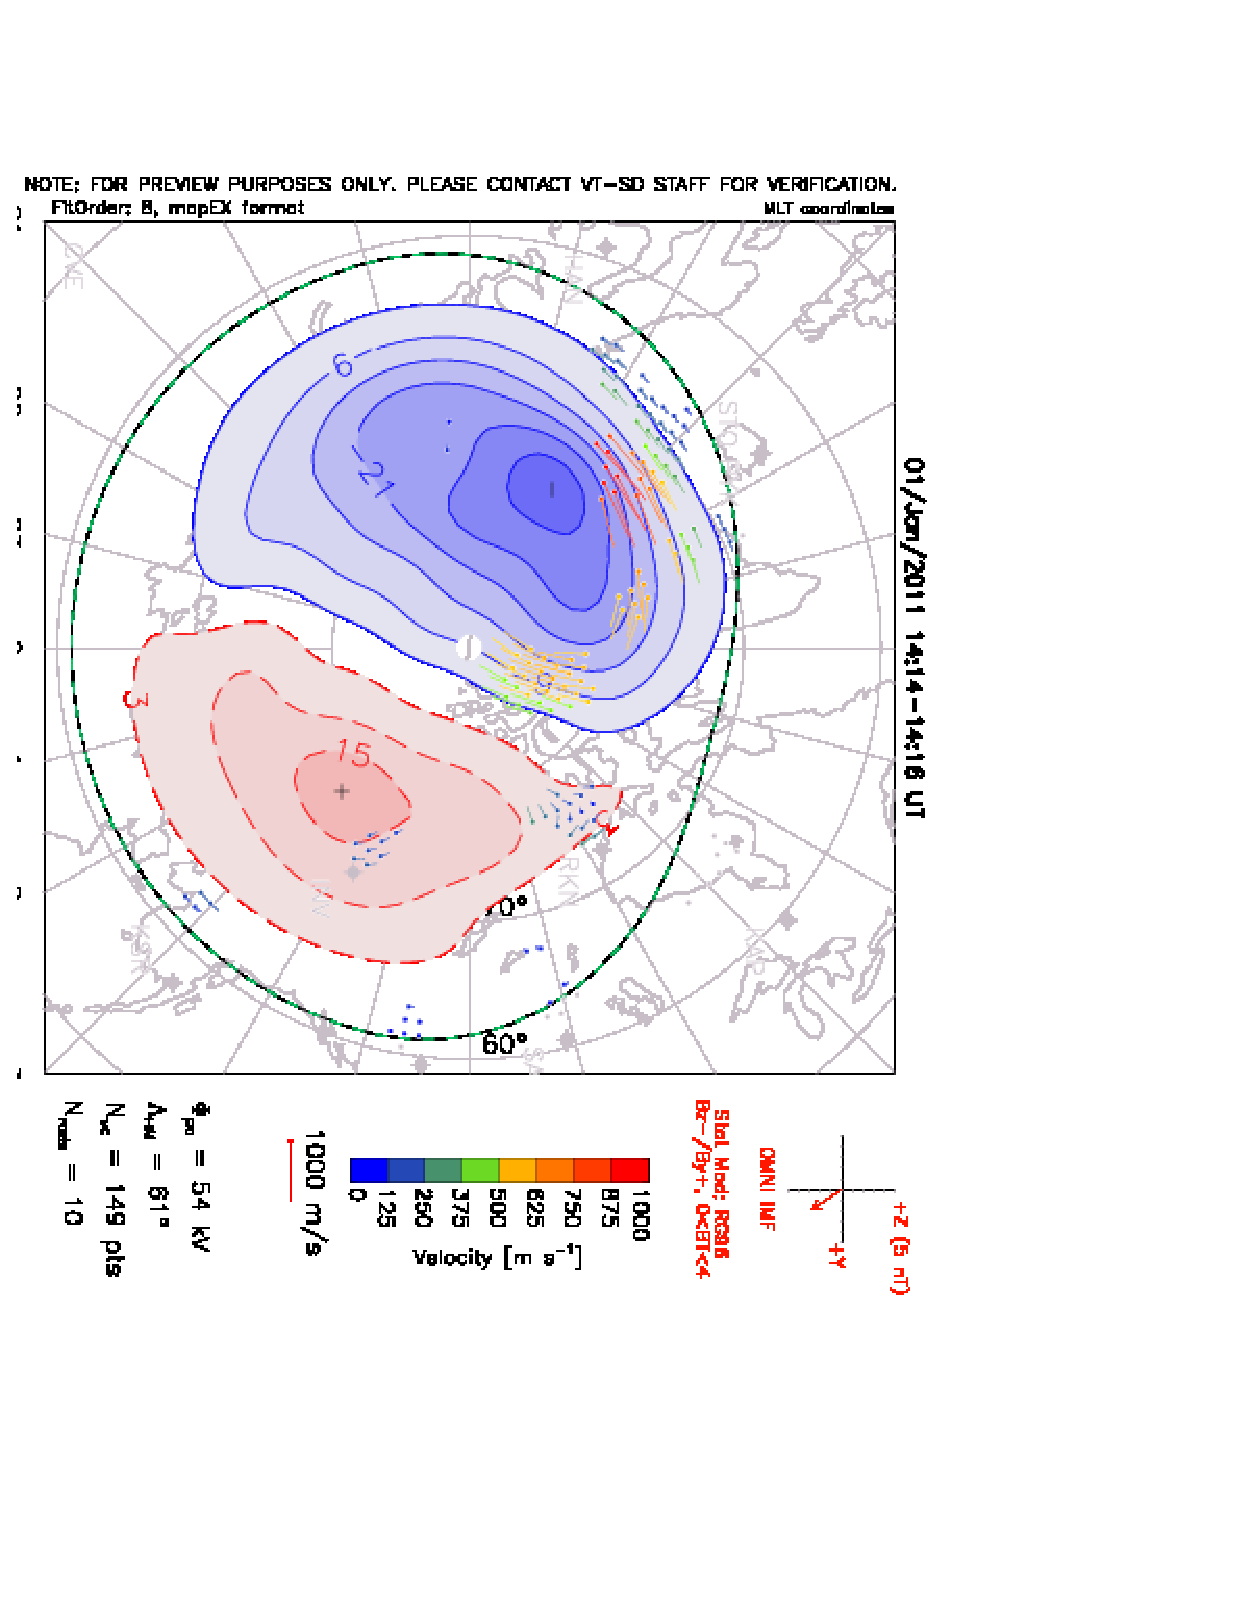
\includegraphics[angle=90,width=\textwidth]{Figures/SD/pot_1415.eps}
\caption{SuperDARN at 14.15}
\label{fig:SD1415}
\end{figure}

\clearpage
\subsection{Current densities (AMPERE)}

In \figref{fig:AMPERE} the current densities from January 1st 2011 between 11.00 to 15.00  calculated from the Irridium satellites are shown. Here the most interesting time is around 14.00 as this is the time with the highest densities. 


\begin{figure}[ht!]

\begin{minipage}{0.33\textwidth}
\includegraphics[width=0.8\textwidth]{Figures/Ampere/1293879600at1100north.pdf}
\caption{11.00}
\end{minipage}
\begin{minipage}{0.33\textwidth}
\includegraphics[width=0.8\textwidth]{Figures/Ampere/1293883200at1200north.pdf}
\caption{12.00}
\end{minipage}
\begin{minipage}{0.33\textwidth}
\includegraphics[width=0.8\textwidth]{Figures/Ampere/1293886800north.pdf}
\caption{13.00}
\end{minipage}

\begin{minipage}{0.33\textwidth}
\includegraphics[width=0.8\textwidth]{Figures/Ampere/1293890400at1400north.pdf}
\caption{14.00}
\end{minipage}
\begin{minipage}{0.33\textwidth}
\includegraphics[width= 0.8\textwidth]{Figures/Ampere/1293891360at1416north.pdf}
\caption{14.16}
\end{minipage}
\begin{minipage}{0.33\textwidth}
\includegraphics[width=0.8\textwidth]{Figures/Ampere/1293894000north.pdf}
\caption{15.00}
\end{minipage}

\caption{Current densities from 11.00 to 16.00 on January 1st 2011, scale from -1.5 $\frac{uA}{m^2}$ to 1.5 $\frac{uA}{m^2}$ , one figure for each hour and an extra for 14.16}
\label{fig:AMPERE}
\end{figure}

At 14.00 the current is up above Svalbard which is the most interesting place to study due to the all-sky camera. And down a bit further south. On the Canadian side there is down furthest north and out further south. At 12.00 there also is a higher density of outward current above Svalbard. 


\subsection{Aurora}

When looking at the Keograms during the day then there is most activity between 11.00 and 15.00. So these will be the ones considered. Starting in the time period between 11.00 and 12.00 then it's possible to see some activity???????

In the keograms the 


\begin{figure}

%%\begin{minipage}{0.49\textwidth}
%%\includegraphics[width = \textwidth]{Figures/Allsky/5577/nya4_20110101_0000_2400_5577_cal.png}
%%\end{minipage}
%%\begin{minipage}{0.49\textwidth}
%%\includegraphics[width=\textwidth]{Figures/Allsky/6300/nya4_20110101_0000_2400_6300_cal.png}
%%\end{minipage}


\begin{minipage}{0.24\textwidth}
\includegraphics[width=\textwidth]{Figures/Allsky/5577/nya4_20110101_1100_1200_5577_cal.png}
\end{minipage}
\begin{minipage}{0.24\textwidth}
\includegraphics[width=\textwidth]{Figures/Allsky/5577/nya4_20110101_1200_1300_5577_cal.png}
\end{minipage}
\begin{minipage}{0.24\textwidth}
\includegraphics[width=\textwidth]{Figures/Allsky/6300/nya4_20110101_1100_1200_6300_cal.png}
\end{minipage}
\begin{minipage}{0.24\textwidth}
\includegraphics[width=\textwidth]{Figures/Allsky/6300/nya4_20110101_1200_1300_6300_cal.png}
\end{minipage}

\begin{minipage}{0.24\textwidth}
\includegraphics[width=\textwidth]{Figures/Allsky/5577/nya4_20110101_1300_1400_5577_cal.png}
\end{minipage}
\begin{minipage}{0.24\textwidth}
\includegraphics[width=\textwidth]{Figures/Allsky/5577/nya4_20110101_1400_1500_5577_cal.png}
\end{minipage}
\begin{minipage}{0.24\textwidth}
\includegraphics[width=\textwidth]{Figures/Allsky/6300/nya4_20110101_1300_1400_6300_cal.png}
\end{minipage}
\begin{minipage}{0.24\textwidth}
\includegraphics[width=\textwidth]{Figures/Allsky/6300/nya4_20110101_1400_1500_6300_cal.png}
\end{minipage}


\caption{Keograms for the time period between 11.00 and 15.00. The four on the left side is in the 5577\AA and the four on the right is in 6300 \AA}
\end{figure}


	\chapter{Discussion}
\label{chap:Discussion}

\section{Interplanetary magnetic field and interaction with Earth's magnetic field.}

As observed on the satellite ACE there is a change in the magnetic field strength, this change to a negative direction is connected to the southward IMF. So there is a burst of plasma coming towards Earth, that will lead to reconnection and an auroral storm. This also means that there are plasma flowing that causes aurora. That there is reconnection is supported by the magnetograms from Svalbard and Bj\o rn \o ya. They show a change in the magnetic field strength a bit more than an hour later. So the solar wind has moved the IMF so that there can be reconnection and it from the data given by the ground-based magnetometers it also seems like that is whats happening. 



This reconnection causes the opened magnetic field lines to move back into the tail. When these magnetic field lines reconnect in the tail again and becomes closed field lines then the plasma can rush down the field lines and cause aurora. Also the magnetic field lines then move to the day side again as a part of the Dungey cycle. 


	\input{Chapters/Conclusion.tex}

	% ¤¤ LITTERATURLISTE: SKAL VÆRE SIDST ¤¤
		\bibliographystyle{ieeetr}
		\bibliography{Bibtex/litteratur}

% ¤¤ BILAG: SKAL VÆRE ALLERSIDST ¤¤
	\appendix

	
\end{document}
